\section{Results}
\label{sec:results}

\begin{figure*}[ht]
  \centering
  \begin{subfigure}[b]{0.48\linewidth}
    \centering
    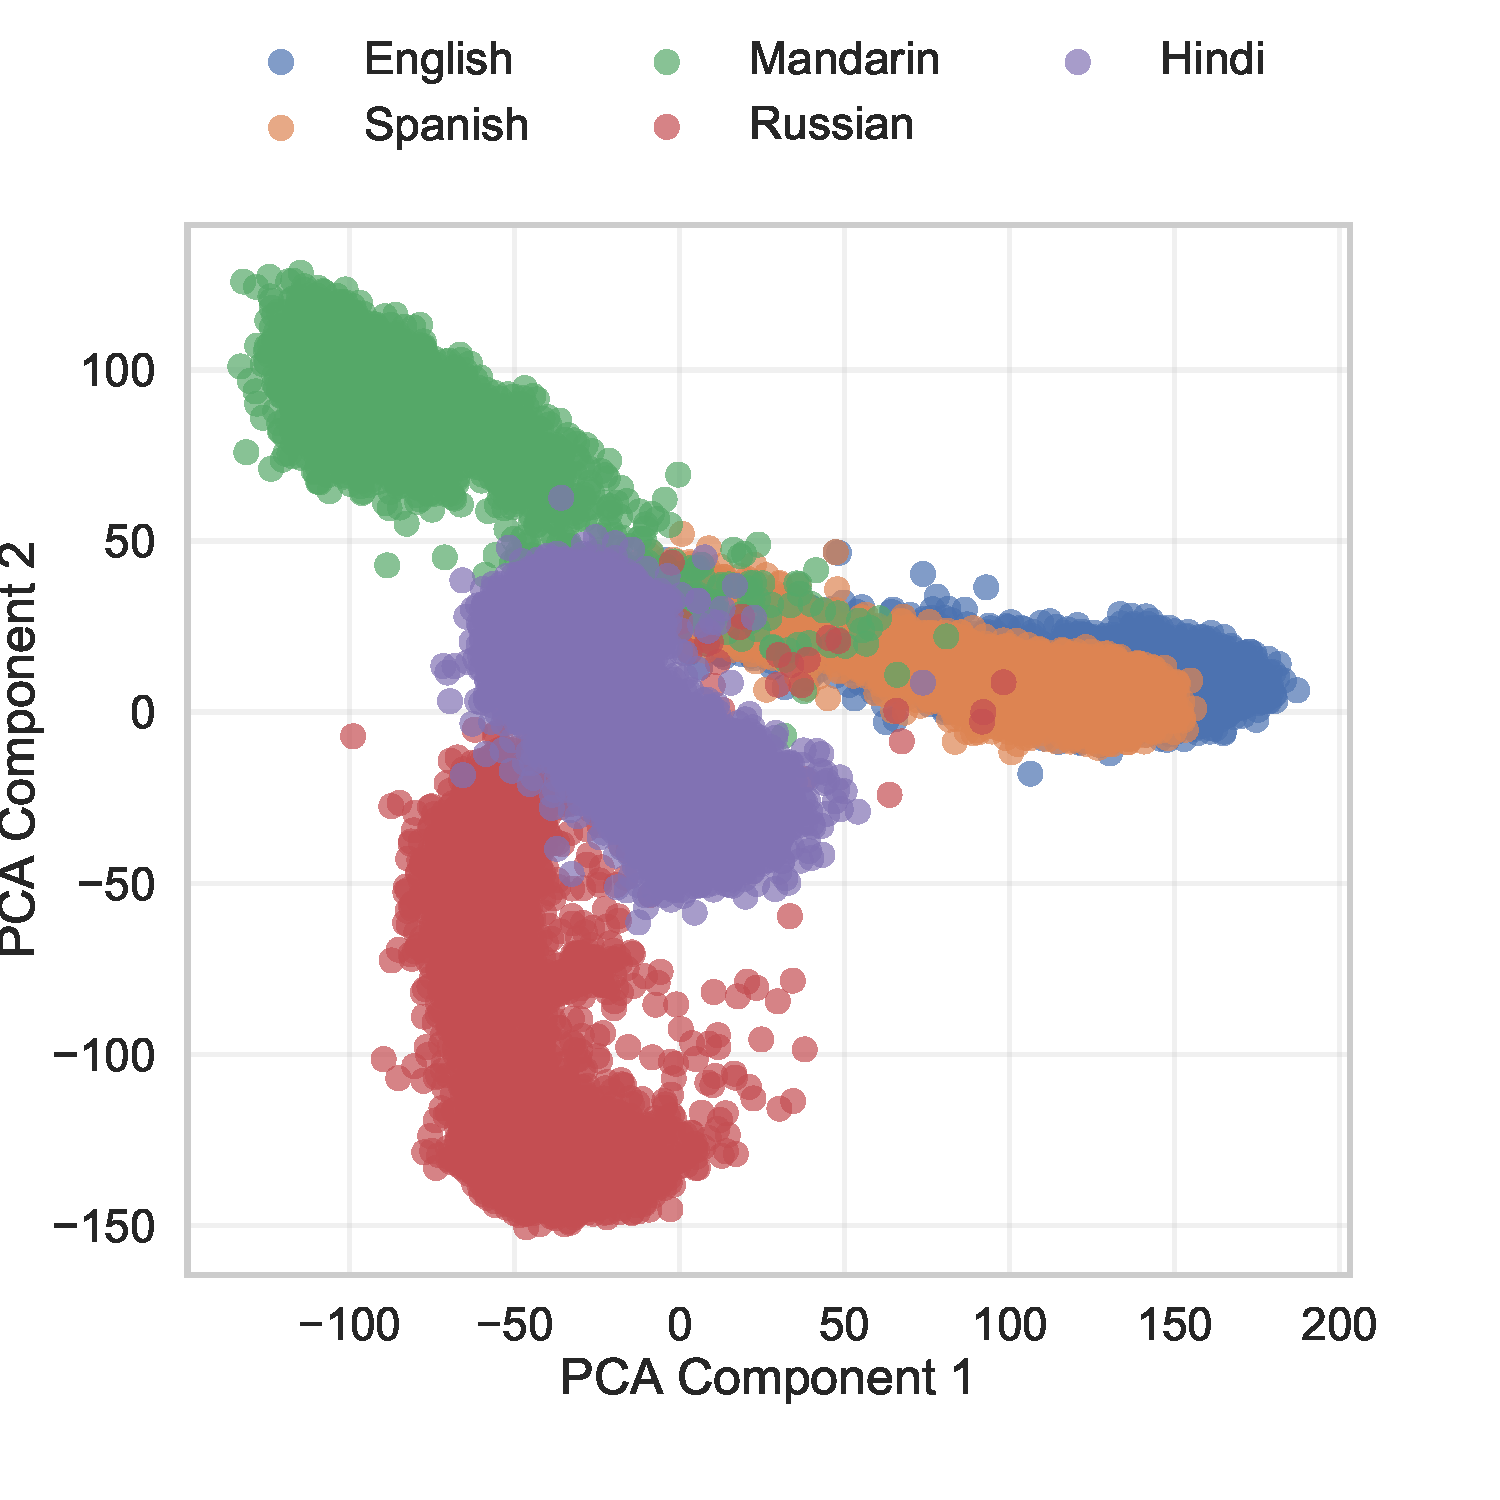
\includegraphics[width=1\linewidth]{images/language_map/multi/qwen/layer_28.pdf}
    \caption{Final layer language map (Qwen)}
    \label{fig:qwen_lang_map}
  \end{subfigure}
  \hfill
  \begin{subfigure}[b]{0.48\linewidth}
    \centering
    
\includegraphics[width=1\linewidth]{images/language_map/multi/llama/layer_16.pdf}
    \caption{Final layer language map (Llama)}
    \label{fig:llama_lang_map}
  \end{subfigure}
\end{figure*}

\begin{figure*}[ht]
  \centering
  \begin{subfigure}[t]{0.24\linewidth}
    \centering
    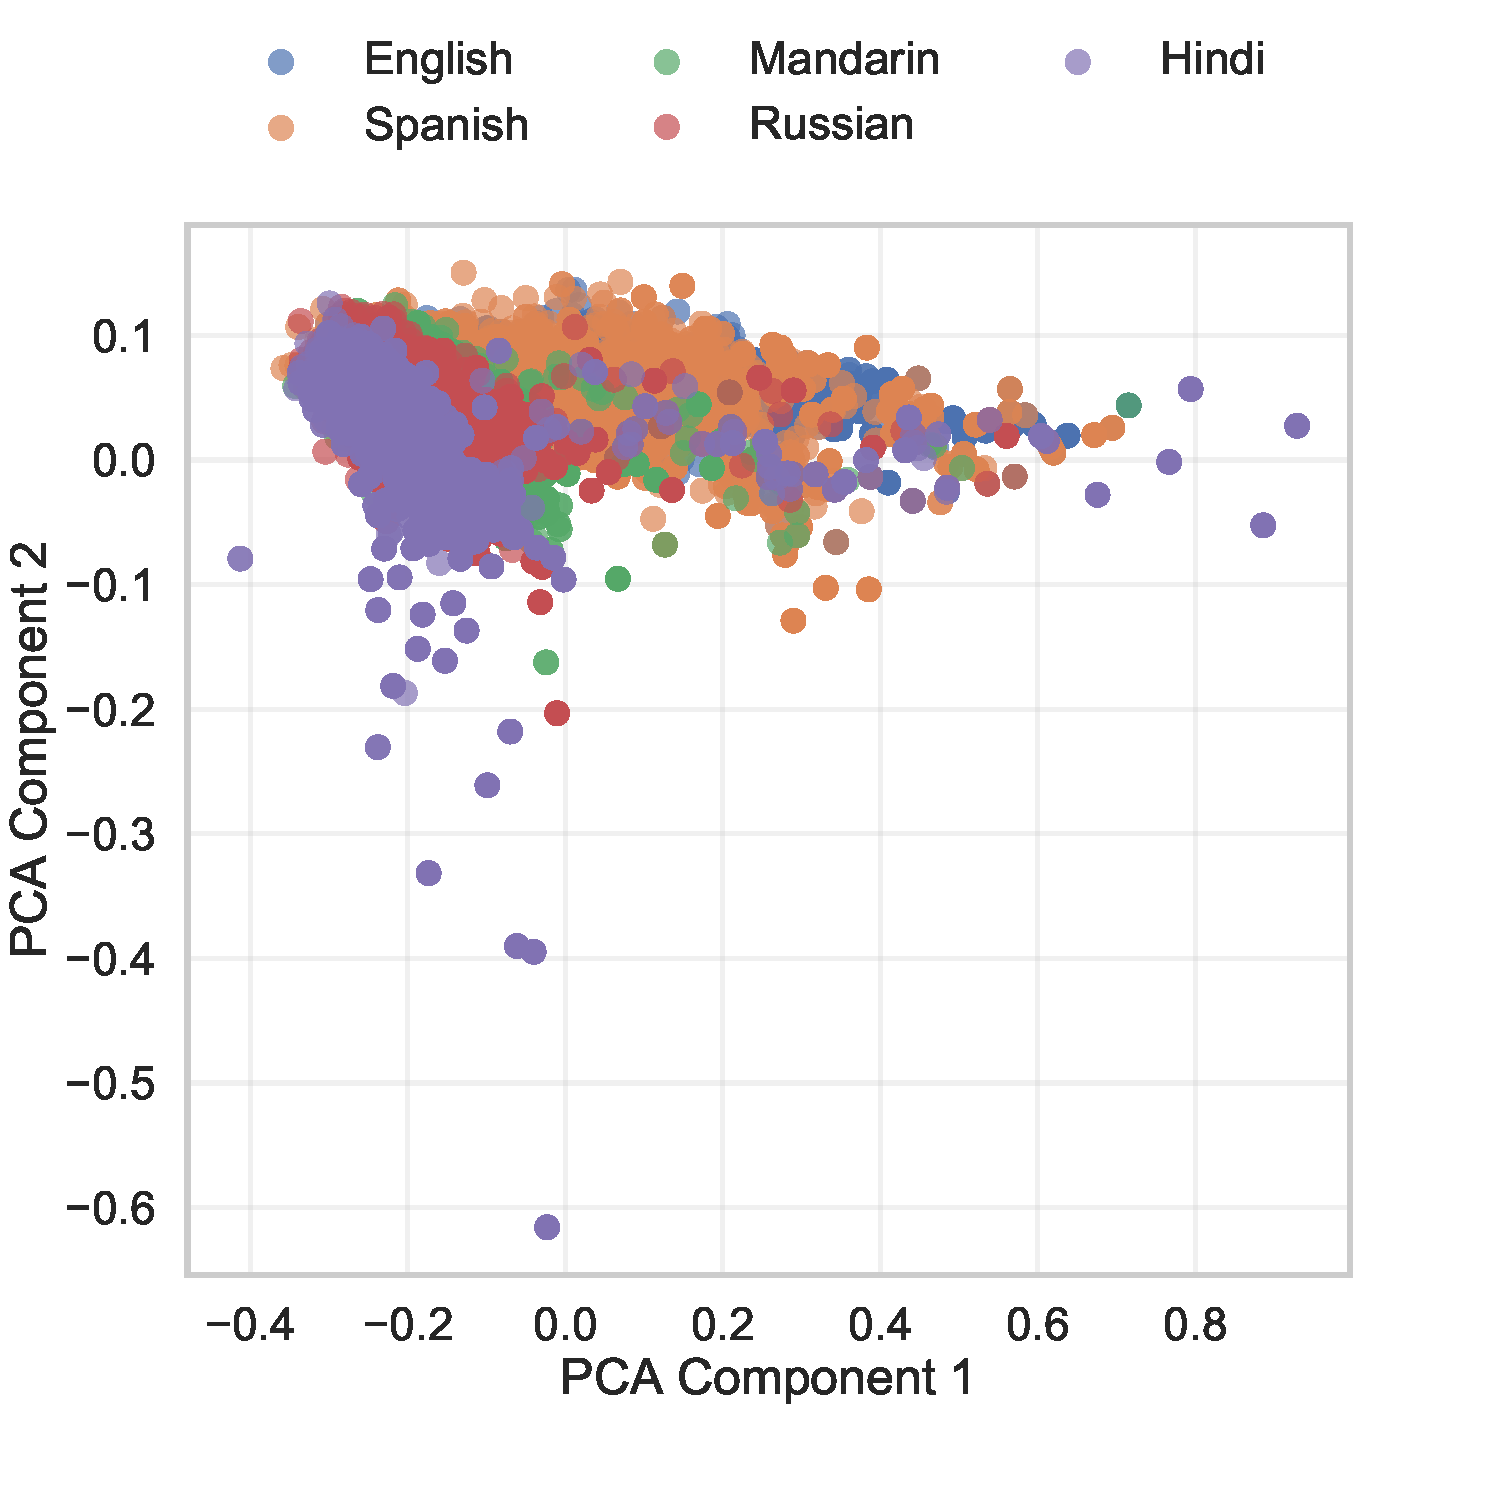
\includegraphics[width=1\linewidth]{images/language_map/multi/llama/layer_0.pdf}
    \caption{First layer language map (Llama)}
    \label{fig:llama_lang_map_first}
  \end{subfigure}
  \hfill
  \begin{subfigure}[t]{0.24\linewidth}
    \centering
    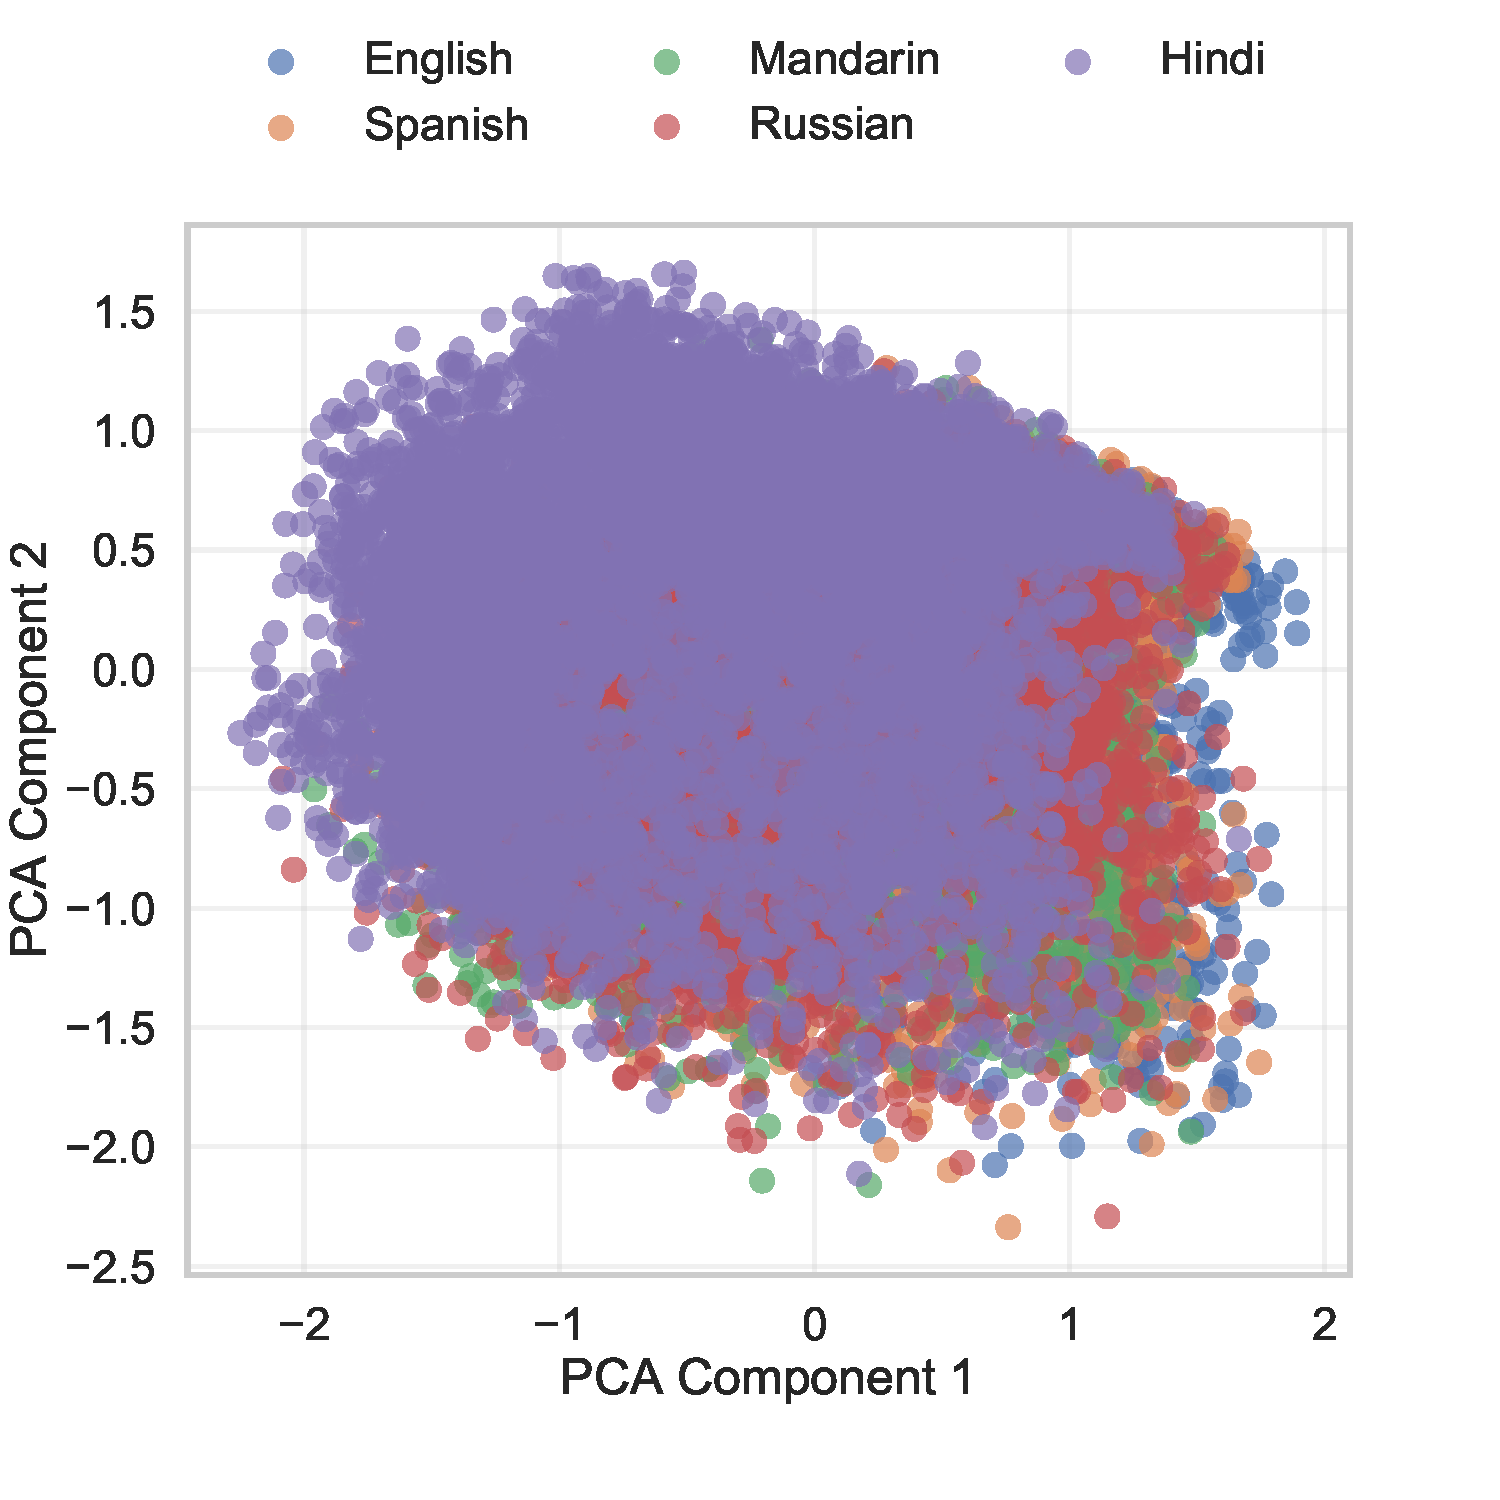
\includegraphics[width=1\linewidth]{images/language_map/multi/llama/layer_7.pdf}
    \caption{Mid-layer language map (Llama)}
    \label{fig:llama_lang_map_mid}
  \end{subfigure}
  \hfill
  \begin{subfigure}[t]{0.48\linewidth}
    \centering
    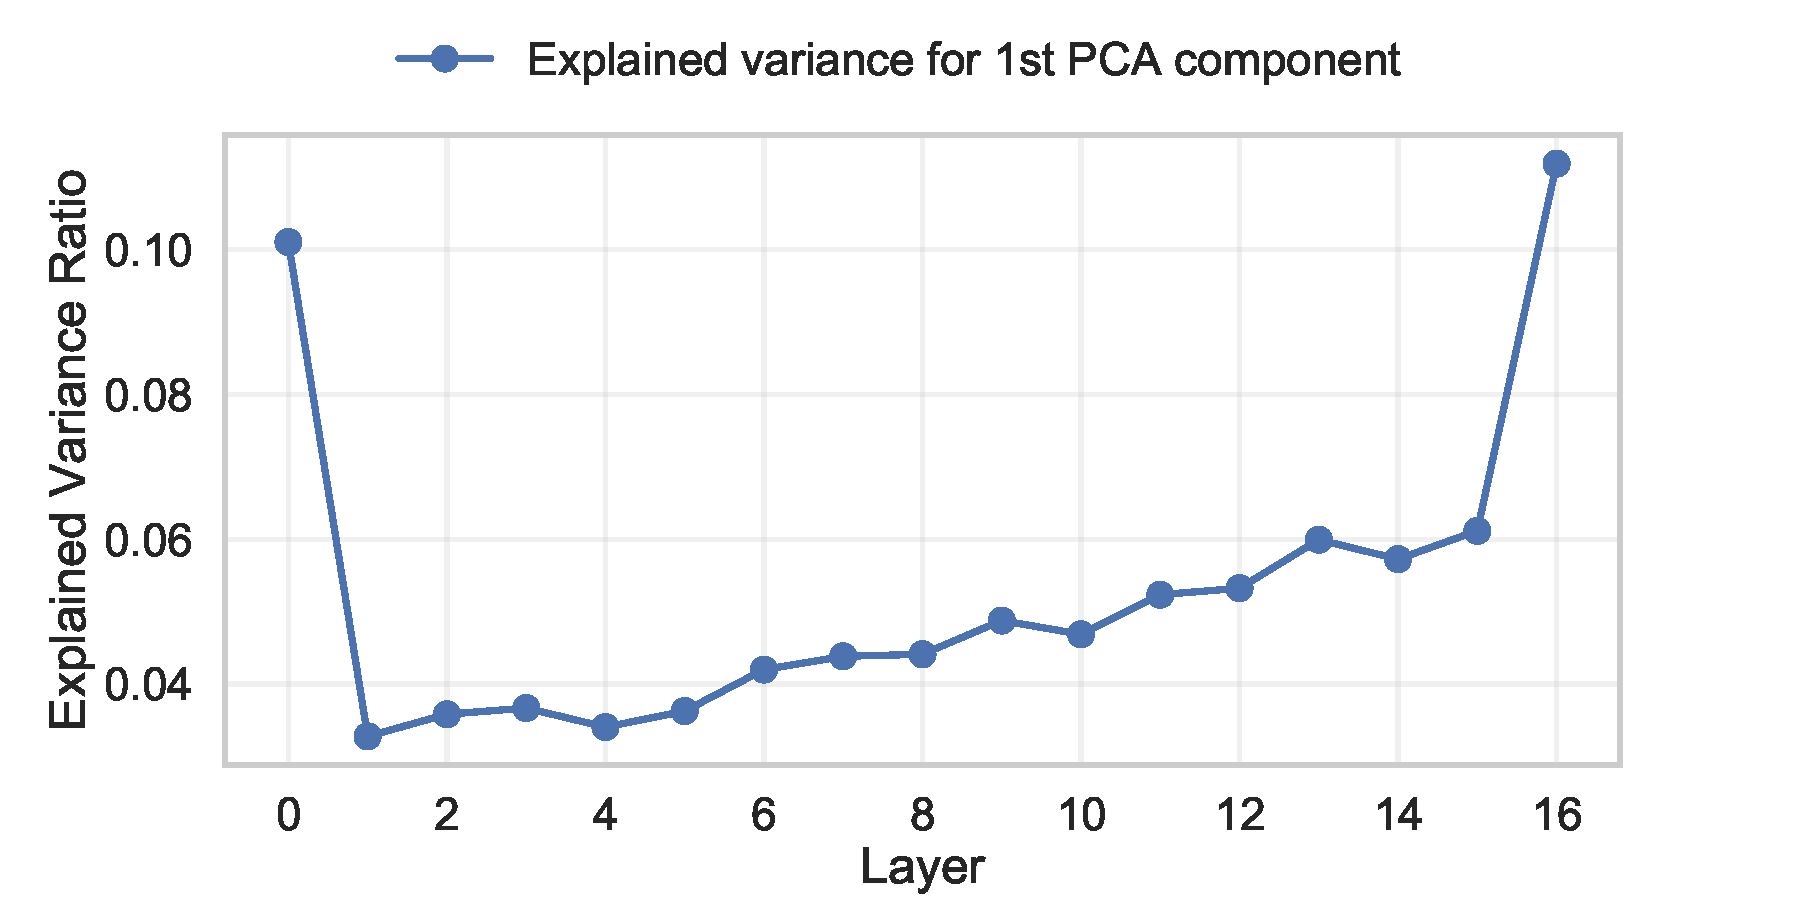
\includegraphics[width=1\linewidth]{images/language_map/multi/llama/explained_variance.pdf}
    \caption{Explained variance (Llama)}
    \label{fig:llama_explained_variance}
  \end{subfigure}
\end{figure*}

\begin{figure*}[ht]
  \centering
  \begin{subfigure}[t]{0.24\linewidth}
    \centering
    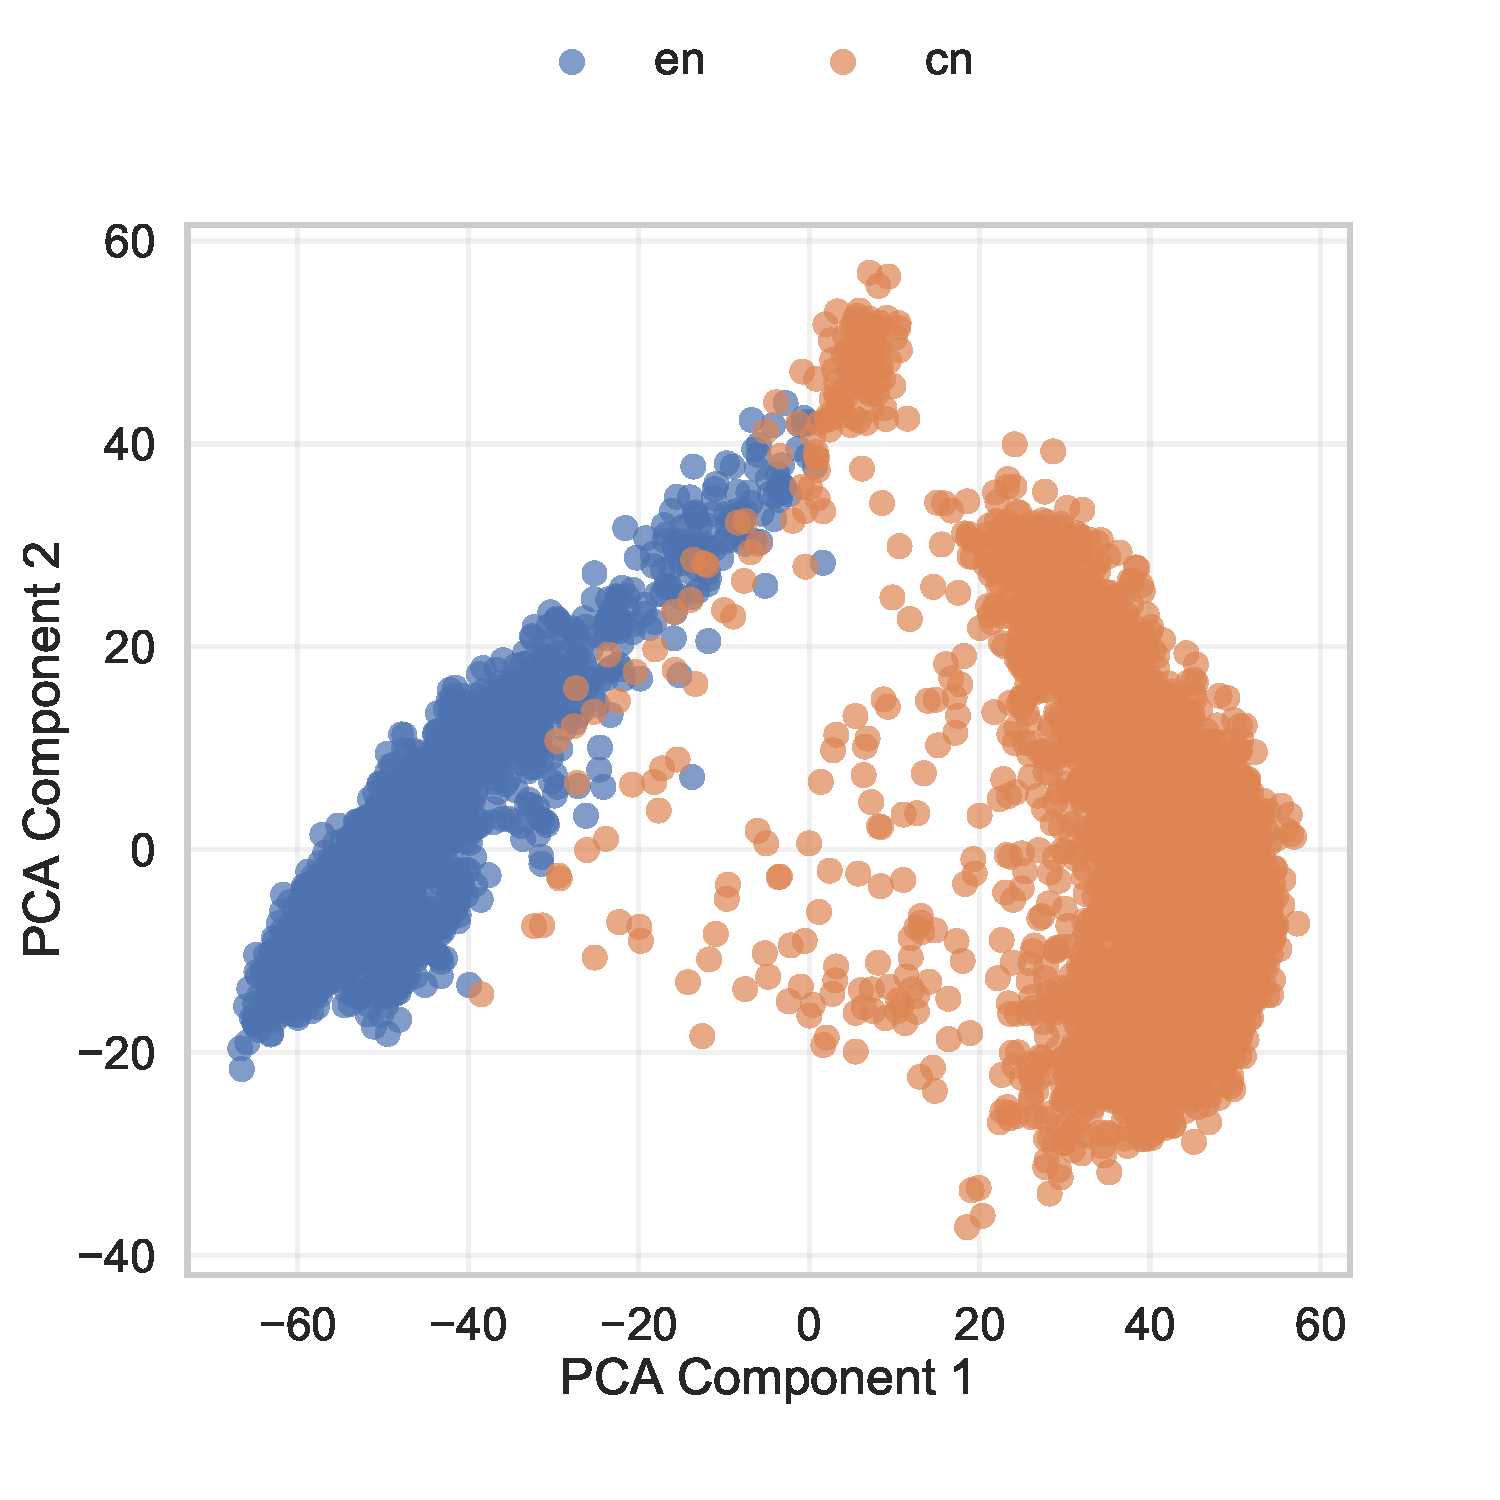
\includegraphics[width=1\linewidth]{images/language_map/en_cn/llama/layer_16.pdf}
    \caption{English - Chinese}
    \label{fig:llama_lang_map_en_cn}
  \end{subfigure}
  \hfill
  \begin{subfigure}[t]{0.24\linewidth}
    \centering
    
\includegraphics[width=1\linewidth]{images/language_map/en_es/llama/layer_16.pdf}
    \caption{English - Spanish}
    \label{fig:llama_lang_map_en_es}
  \end{subfigure}
  \hfill
  \begin{subfigure}[t]{0.24\linewidth}
    \centering
    
\includegraphics[width=1\linewidth]{images/language_map/en_ru/llama/layer_16.pdf}
    \caption{English - Russian}
    \label{fig:llama_lang_map_en_ru}
  \end{subfigure}
  \hfill
  \begin{subfigure}[t]{0.24\linewidth}
    \centering
    
\includegraphics[width=1\linewidth]{images/language_map/en_hin/llama/layer_16.pdf}
    \caption{English - Hindi}
    \label{fig:llama_lang_map_en_hin}
  \end{subfigure}
\end{figure*}

We validate our approach on Qwen2.5-1.5B ~\cite{qwen2025qwen25technicalreport} and Llama-3.2-1B ~\cite{grattafiori2024llama3herdmodels} open models across multiple language pairs, demonstrating both the existence of interpretable language directions and their effectiveness for code-switching control.

\subsection{Language direction identification}

\paragraph{Experimental setup.} We use Flores Plus \cite{nllb-24} dataset with 50 parallel samples (English, Spanish, Russian, Chinese, Hindi) for PCA fitting and 100 for validation.

\paragraph{Language maps reveal emergent clustering.} Figure~\ref{fig:qwen_lang_map} and~\ref{fig:llama_lang_map} show final-layer embeddings projected onto the first two PCs. Consistent with prior findings~\cite{conneau-etal-2020-emerging, wendler-etal-2024-llamas}, models organize identical content into tight, language-specific clusters with clear boundaries. Languages within the Indo-European family (Spanish, Russian) cluster closer than typologically distant pairs (English--Chinese), suggesting PC1 captures coarse language distinction while PC2 encodes finer linguistic properties.

Figures ~\ref{fig:llama_lang_map_first} ~\ref{fig:llama_lang_map_mid} show layer-wise evolution: clusters emerge loosely in early layers and sharpen dramatically in final layers. Figure~\ref{fig:llama_explained_variance} reveals late-stage specialization for language identity. Pairwise maps (Figures ~\ref{fig:llama_lang_map_en_cn}, ~\ref{fig:llama_lang_map_en_es}, ~\ref{fig:llama_lang_map_en_ru}, ~\ref{fig:llama_lang_map_en_hin}) confirm clean linear separability for all tested pairs.

\subsection{Language prediction}

\paragraph{Experimental setup.} We use Flores Plus \cite{nllb-24} dataset with 50 parallel samples (English, Spanish, Russian, Chinese, Hindi) for PCA and logistic regression fitting and 100 for validation.
\paragraph{Classifier shows nearly perfect performance.} Table~\ref{tab:clf} demonstrates that a simple logistic regression classifier trained only on the first principal component achieves near-perfect accuracy (0.96-1.00) across all language pairs and both models. This validates that language identity information is linearly accessible in the final layer representations, supporting our hypothesis that models maintain explicit language directions in their activation space. We observe decreased performance for the English-Spanish pair in both models, attributable to these languages being more closely related to each other.

\begin{table}[h]
  \centering
  \begin{tabular}{l l l}
    \hline
    Language pair & Qwen & Llama \\
    \hline
    English - Chinese & 0.98 & 0.98 \\
    English - Spanish & 0.96 & 0.96 \\
    English - Russian & 0.99 & 0.99 \\
    English - Hindi & 0.98 & 1.00 \\
    \hline
  \end{tabular}
  \caption{Last layer language classifier accuracy}
  \label{tab:clf}
\end{table}

\subsection{Language steering}

\paragraph{Experimental setup.} We fit the steering module on Flores Plus with 200 parallel samples and test on 2,467 TED Talks samples with artificial code-switching. Each sample is truncated to 20 words, split at the midpoint, and the second half is translated to the target language using Gemini 2.5 Flash via the OpenRouter API, producing texts that begin in English and switch mid-sentence. We note that this artificial code-switchin created by translating the second half of each sentence may not capture the full complexity of naturally occurring code-switching. We use this controlled setup to isolate the effect of steering but acknowledge the need for evaluation on naturally occurring code-switched text in future work. Success is measured by comparing the next-token prediction distribution of the steered model against the English baseline using four complementary metrics: KL divergence $\text{KL}(P_{\text{EN}} \| P_{\text{steered}})$, Jensen-Shannon divergence, cosine similarity, and top-50 token overlap. Lower divergence and higher similarity/overlap indicate better mitigation.

To find the best steering strength coefficient we conduct a grid search with the best values listed in Table~\ref{tab:steering_coeff} for each language pair.

\begin{table}[h]
  \small
  \centering
  \begin{tabular}{l l l}
    \hline
    Original & Unsteered & Steered \\
    \hline
    still & muy & very \\
    going & un  & surprised \\
    not & bastante & pretty \\
    so & tan & starting \\
    a & sor & working \\
    just & más & content \\
    really & a & rather \\
    in & empez & impressed \\
    very & de & quite \\
    sitting & content & -- \\
    quite & en & great \\
    pretty & enc & beginning \\
    here & aquí & answering \\
    thinking & pens & almost\\
    looking & realmente & fully \\
    kind & dese & \_\_\_\_ \\
    getting & completamente & \_\_ \\
    having & feliz & even \\
    actually & org & heart \\
    surprised & seguro & trying \\
    \hline
  \end{tabular}
  \caption{Top 20 token sample (Qwen, English-Spanish)}
  \label{tab:token_sample}
\end{table}

\paragraph{Results.} Table~\ref{tab:token_sample} demonstrates that steering shifts predictions from Spanish tokens (muy, bastante, tan) to their English equivalents (very, quite, so) while preserving semantic coherence. For well-calibrated coefficients, steering changes \emph{how} the model speaks rather than \emph{what} it says, though aggressive coefficients can disrupt semantic content (see Limitations).

Table~\ref{tab:kl} shows steering reduces KL divergence by 25-55\% across language pairs and models (38\% average for Qwen, 43\% for Llama). While the method substantially mitigates code-switching, the remaining gap indicates that the complex structure of the manifold does not allow full reconstruction of the original concept with a simple linear transformation. The method shows strongest performance for typologically distant pairs: English-Chinese achieves 55\% KL reduction on Qwen, while English-Russian achieves 55\% on Llama. We hypothesize that model-specific tokenization and training data balance play a key role: the Qwen model processed much more English and Chinese data, leading to more granular tokenization and better internal generalization for that pair. English-Hindi remains the weakest pair for both models (24-27\% reduction).

These findings are supported by supplementary metrics. JS divergence (Table~\ref{tab:js}) shows consistent improvement across all pairs. Cosine similarity between steered and English baseline distributions increases substantially (Table~\ref{tab:cos}), e.g., from 0.02 to 0.22 for Qwen English-Chinese. Top-50 token overlap (Table~\ref{tab:overlap}) reveals that steering dramatically increases the number of shared high-probability tokens with the English baseline - from under 8\% to over 25\% for most pairs. English-Hindi on Qwen again shows minimal improvement across all supplementary metrics (cosine: 0.04 $\rightarrow$ 0.07, overlap: 11.23\% $\rightarrow$ 11.68\%), reinforcing that this is the most challenging pair.

Notably, the optimal steering coefficient for Qwen English-Hindi is positive ($+5.0$), indicating a reversed PCA direction for this pair relative to all others. This may reflect tokenization asymmetries in the Qwen model's treatment of Devanagari script. In contrast, Llama uses a consistent negative direction across all language pairs (Table~\ref{tab:steering_coeff}).

\begin{table}[h]
  \centering
  \begin{tabular}{l l l}
    \hline
    Language pair & Qwen & Llama \\
    \hline
    English - Chinese & 10.15 $\rightarrow$ 4.52 & 9.05 $\rightarrow$ 4.77 \\
    English - Spanish & 7.25 $\rightarrow$ 4.90 & 6.52 $\rightarrow$ 3.48 \\
    English - Russian & 8.70 $\rightarrow$ 5.40 & 7.77 $\rightarrow$ 3.49 \\
    English - Hindi & 9.60 $\rightarrow$ 7.02 & 8.06 $\rightarrow$ 6.13 \\
    \hline
  \end{tabular}
  \caption{KL divergence (no steering $\rightarrow$ steering)}
  \label{tab:kl}
\end{table}

\begin{table}[h]
  \centering
  \begin{tabular}{l l l}
    \hline
    Language pair & Qwen & Llama \\
    \hline
    English - Chinese & 0.67 $\rightarrow$ 0.49 & 0.65 $\rightarrow$ 0.51 \\
    English - Spanish & 0.59 $\rightarrow$ 0.52 & 0.58 $\rightarrow$ 0.44 \\
    English - Russian & 0.62 $\rightarrow$ 0.50 & 0.62 $\rightarrow$ 0.43 \\
    English - Hindi & 0.64 $\rightarrow$ 0.60 & 0.63 $\rightarrow$ 0.54 \\
    \hline
  \end{tabular}
  \caption{JS divergence (no steering $\rightarrow$ steering)}
  \label{tab:js}
\end{table}

\begin{table}[h]
  \centering
  \begin{tabular}{l l l}
    \hline
    Language pair & Qwen & Llama \\
    \hline
    English - Chinese & 0.02 $\rightarrow$ 0.22 & 0.05 $\rightarrow$ 0.21 \\
    English - Spanish & 0.12 $\rightarrow$ 0.18 & 0.12 $\rightarrow$ 0.29 \\
    English - Russian & 0.09 $\rightarrow$ 0.23 & 0.10 $\rightarrow$ 0.31 \\
    English - Hindi & 0.04 $\rightarrow$ 0.07 & 0.06 $\rightarrow$ 0.16 \\
    \hline
  \end{tabular}
  \caption{Cosine similarity (no steering $\rightarrow$ steering, higher = better)}
  \label{tab:cos}
\end{table}

\begin{table}[h]
  \centering
  \begin{tabular}{l l l}
    \hline
    Language pair & Qwen & Llama \\
    \hline
    English - Chinese & 3.69\% $\rightarrow$ 26.46\% & 4.47\% $\rightarrow$ 24.31\% \\
    English - Spanish & 11.41\% $\rightarrow$ 20.23\% & 11.45\% $\rightarrow$ 30.74\% \\
    English - Russian & 7.41\% $\rightarrow$ 25.45\% & 7.49\% $\rightarrow$ 31.96\% \\
    English - Hindi & 11.23\% $\rightarrow$ 11.68\% & 6.54\% $\rightarrow$ 25.88\% \\
    \hline
  \end{tabular}
  \caption{Top-50 token overlap (no steering $\rightarrow$ steering, higher = better)}
  \label{tab:overlap}
\end{table}

\begin{table}[h]
  \centering
  \begin{tabular}{l l l}
    \hline
    Language pair & Qwen & Llama \\
    \hline
    English - Chinese & $-3.2$ & $-5.0$ \\
    English - Spanish & $-2.8$ & $-3.7$ \\
    English - Russian & $-2.2$ & $-3.5$ \\
    English - Hindi & $+5.0$ & $-3.6$ \\
    \hline
  \end{tabular}
  \caption{Best steering strength coefficient (KL-optimized)}
  \label{tab:steering_coeff}
\end{table}

\subsection{Generation-based evaluation}
\label{sec:generation_eval}

To complement the distributional analysis above, we evaluate steering on actual text generation using Llama-3.2-1B. For each of 500 TED Talks samples per language pair, we generate 100-token continuations in three conditions: (A)~English-only input without steering, (B)~code-switched input without steering, and (C)~code-switched input with steering. We measure code-switching in the generated output using standard metrics~\cite{gamback-das-2016-comparing, guzman17_interspeech}: \emph{Code-Switching Index} (CSI), the fraction of tokens not in the target language (lower = better); \emph{M-Index}, a multilingual diversity measure ($0$ = monolingual, $1$ = maximally mixed); \emph{I-Index}, the ratio of language switch points to token boundaries; and \emph{Target Language Consistency} (TLC $= 1 - \text{CSI}$, higher = better). Token-level language identification uses a FastText classifier with a sliding window of 5 tokens.

\paragraph{Steering coefficients.} We evaluate two sets of steering coefficients (Table~\ref{tab:steering_coeff_gen}). The \emph{KL-optimized} set uses the coefficients from the distributional grid search (Table~\ref{tab:steering_coeff}). The \emph{CSI-optimized} set is obtained by a separate grid search that directly minimizes CSI on a 10-sample calibration subset. CSI-optimized coefficients tend toward higher magnitudes, which improves language control but increases degeneration risk (see Limitations).

\begin{table}[h]
  \centering
  \begin{tabular}{l c c}
    \hline
    Language pair & KL-opt. & CSI-opt. \\
    \hline
    English - Chinese  & $-5.0$ & $-5.0$ \\
    English - Spanish  & $-3.7$ & $-5.0$ \\
    English - Russian  & $-3.5$ & $-4.0$ \\
    English - Hindi    & $-3.6$ & $-5.0$ \\
    \hline
  \end{tabular}
  \caption{Llama-3.2-1B steering coefficients: KL-optimized (from distributional analysis) vs.\ CSI-optimized (from generation grid search).}
  \label{tab:steering_coeff_gen}
\end{table}

\paragraph{Results.} Table~\ref{tab:gen_results} shows that steering substantially reduces code-switching in generated text. With KL-optimized coefficients, CSI drops by 63--95\% across language pairs, demonstrating that distributional optimization transfers well to generation. CSI-optimization yields further gains for English-Spanish ($0.23 \rightarrow 0.11$) and English-Hindi ($0.04 \rightarrow 0.01$), but at the cost of higher-magnitude coefficients that increase degeneration risk.

\begin{table}[h]
  \centering
  \small
  \begin{tabular}{l c c c c}
    \hline
    & \multicolumn{2}{c}{KL-optimized} & \multicolumn{2}{c}{CSI-optimized} \\
    \cmidrule(lr){2-3} \cmidrule(lr){4-5}
    Language pair & CSI ($\downarrow$) & TLC ($\uparrow$) & CSI ($\downarrow$) & TLC ($\uparrow$) \\
    \hline
    \multicolumn{5}{l}{\textit{Unsteered (code-switched input, no steering):}} \\
    English - Chinese  & \multicolumn{2}{c}{0.64 / 0.36} & \multicolumn{2}{c}{---} \\
    English - Spanish  & \multicolumn{2}{c}{0.62 / 0.38} & \multicolumn{2}{c}{---} \\
    English - Russian  & \multicolumn{2}{c}{0.59 / 0.41} & \multicolumn{2}{c}{---} \\
    English - Hindi    & \multicolumn{2}{c}{0.81 / 0.19} & \multicolumn{2}{c}{---} \\
    \hline
    \multicolumn{5}{l}{\textit{Steered:}} \\
    English - Chinese  & 0.03 & 0.97 & 0.03 & 0.97 \\
    English - Spanish  & 0.23 & 0.77 & 0.11 & 0.89 \\
    English - Russian  & 0.02 & 0.98 & 0.01 & 0.99 \\
    English - Hindi    & 0.04 & 0.96 & 0.01 & 0.99 \\
    \hline
  \end{tabular}
  \caption{Generation-based code-switching metrics (Llama-3.2-1B, $n=500$). English-only baseline: CSI~$= 0.02$. All steered vs.\ unsteered differences significant at $p < 0.001$ (Wilcoxon signed-rank test).}
  \label{tab:gen_results}
\end{table}

Notably, steering coefficients are highly fragile: small changes in magnitude can shift the model from fluent code-switched output to degenerate repetition. The CSI-optimized coefficients cluster near the maximum tested value ($-5.0$), suggesting that direct optimization of generation metrics pushes toward an aggressive regime where language control and fluency trade off sharply.

\paragraph{Qualitative analysis.} Table~\ref{tab:qualitative} shows representative examples. Steering successfully redirects generation from the foreign language to English, but aggressive coefficients can produce repetitive output patterns, indicating a trade-off between language control and generation fluency that we discuss further in Limitations.

\begin{table}[h]
  \centering
  \small
  \begin{tabular}{p{0.14\linewidth} p{0.80\linewidth}}
    \hline
    \multicolumn{2}{l}{\textbf{en-es:} \textit{``...I took on the task to ense\~{n}ar desarrollo global...''}} \\
    \hline
    Unsteered & \textit{de que un grupo de estudiantes suecos, que hab\'{i}an sido enviados a la Universidad de Harvard, me escribieron para pedir ayuda...} \\
    Steered & \textit{de that I had the opportunity to work with the first two editions of the course and I was very inspired by it...} \\
    \hline
    \multicolumn{2}{l}{\textbf{en-ru:} \textit{``...About 10 years ago, I took on the task to} [Russian text]\textit{...''}} \\
    \hline
    Degenerate steered & \textit{first year of the first year of the first year of the first year of the first year...} \\
    \hline
  \end{tabular}
  \caption{Generated continuations (Llama-3.2-1B, KL-optimized). Top: steering successfully redirects Spanish to coherent English. Bottom: steering eliminates Russian but produces degenerate repetition.}
  \label{tab:qualitative}
\end{table}